
\documentclass[11pt]{beamer}

% Packages ====================================================================
\usepackage{arev}
\usepackage[T1]{fontenc}
\usepackage[utf8]{inputenc}
\usepackage{float, afterpage, rotating, graphicx}
\usepackage{epstopdf}
\usepackage{longtable, booktabs, tabularx}
\usepackage{fancyvrb, moreverb, relsize}
\usepackage{eurosym, calc, chngcntr}
\usepackage{amsmath, amssymb, amsfonts, amsthm}
\usepackage{xcolor}
\usepackage{verbatim}
\usepackage{setspace}
\usepackage{appendixnumberbeamer}
\usepackage{subcaption}
\usepackage{ragged2e}
\usepackage[backend=biber, natbib=true, bibencoding=inputenc, bibstyle=authoryear-ibid, citestyle=authoryear-comp, maxcitenames=3, maxbibnames=10]{biblatex}
\setlength{\bibitemsep}{1.5ex}
\addbibresource{../../../refs.bib}
\hypersetup{colorlinks=true, linkcolor=., anchorcolor=., citecolor=., filecolor=., menucolor=., runcolor=., urlcolor=.}

% Commands =====================================================================
\DeclareMathOperator*{\argmin}{argmin}
\DeclareMathOperator*{\argmax}{arg\,max}
\renewcommand{\vec}[1]{\mathbf{#1}}
\def\newblock{\hskip .11em plus .33em minus .07em}
\newcommand{\bs}{\boldsymbol}
\newcommand{\N}{\mathbb{N}}
\newcommand{\cov}{\mathrm{cov}\thin}
\newcommand{\thin}{\thinspace}
\newcommand{\thick}{\thickspace}
\newcommand{\Lim}[1]{\raisebox{0.5ex}{\scalebox{0.8}{$\displaystyle \lim_{#1}\;$}}}
\newcommand{\vect}[1]{\mathbf{#1}}
\newcommand{\myfrac}[3][0pt]{\genfrac{}{}{}{}{\raisebox{#1}{$#2$}}{\raisebox{-#1}{$#3$}}}
\newcommand{\U}{\mathrm{U}} %Uniform Distribution
\newcommand{\D}{\mathrm{D}} %Dirichlet Distribution
\newcommand{\W}{\mathrm{W}} %Wishart Distribution
\newcommand{\E}{\mathrm{E}}     %Expectation
\newcommand{\Prob}{\mbox{Pr}}       %Expectation
\newcommand{\Iden}{\mathbb{I}}  %Identity Matrix
\newcommand{\Ind}{\mathrm{I}}   %Indicator Function
\newcommand{\Tau}{\mathcal{T}\thin}
\newcommand{\var}{\mathrm{var}\thin}
\newcommand{\plim}{\mathrm{plim}\thin}
\newcommand\indep{\protect\mathpalette{\protect\independenT}{\perp}}
\def\independenT#1#2{\mathrel{\rlap{$#1#2$}\mkern5mu{#1#2}}}
\newcommand{\notindep}{\ensuremath{\perp\!\!\!\!\!\!\diagup\!\!\!\!\!\!\perp}}%
\newcommand{\mc}{\multicolumn}
\newcommand{\ph}{\phantom}

\newcommand\Wider[2][3em]{%
\makebox[\linewidth][c]{%
  \begin{minipage}{\dimexpr\textwidth+#1\relax}
  \raggedright#2
  \end{minipage}%
  }%
}

\usepackage{minted}

\newminted{python}{fontsize=\tiny,
                   %linenos,
                   numbersep=8pt,
                   gobble=4,
                   %frame=lines,
                   framesep=3mm}

% Colors =======================================================================
% short color names
% blues
\definecolor{lb}{HTML}{3498DB}
\definecolor{b}{HTML}{1565C0}
\definecolor{db}{HTML}{002080}
% greens
\definecolor{lg}{HTML}{B2EC5D}
\definecolor{g}{HTML}{55A868}
\definecolor{dg}{HTML}{2E7D32}
% yellows
\definecolor{ly}{HTML}{F9A825}
\definecolor{y}{HTML}{FF8F00}
\definecolor{dy}{HTML}{EF6C00}
% reds
\definecolor{lr}{HTML}{D84315}
\definecolor{r}{HTML}{C44E52}
\definecolor{dr}{HTML}{C62828}
% violet
\definecolor{lv}{HTML}{C71585}
\definecolor{v}{HTML}{9B59B6}
\definecolor{dv}{HTML}{6A1B9A}
% grey
\definecolor{ln}{HTML}{BDBDBD}
\definecolor{n}{HTML}{757575}
\definecolor{dn}{HTML}{616161}
% palettes
\definecolor{p1}{HTML}{4A6FAC}
\definecolor{p2}{HTML}{53A465}
\definecolor{p3}{HTML}{C04C50}
\definecolor{p4}{HTML}{7E6FAE}
\definecolor{p5}{HTML}{C8B571}
\definecolor{p6}{HTML}{62B1C8}
% brown
\definecolor{brown}{HTML}{4E342E}

% long color names
\definecolor{mm-lightblue}{HTML}{3498DB}
\definecolor{md-lightblue}{HTML}{0277BD}
\definecolor{mm-blue}{HTML}{002080}
\definecolor{md-blue}{HTML}{1565C0}
\definecolor{md-indigo}{HTML}{283593}

\definecolor{md-lime}{HTML}{9E9D24}
\definecolor{mm-lightgreen}{HTML}{B2EC5D}
\definecolor{md-lightgreen}{HTML}{558B2F}
\definecolor{mm-green}{HTML}{55A868}
\definecolor{md-green}{HTML}{2E7D32}
\definecolor{md-teal}{HTML}{00695C}

\definecolor{md-yellow}{HTML}{F9A825}
\definecolor{mm-gold}{HTML}{FFBF00}
\definecolor{md-amber}{HTML}{FF8F00}
\definecolor{md-orange}{HTML}{EF6C00}
\definecolor{md-deeporange}{HTML}{D84315}

\definecolor{mm-red}{HTML}{C44E52}
\definecolor{md-red}{HTML}{C62828}
\definecolor{violetred}{HTML}{C71585}

\definecolor{md-brown}{HTML}{4E342E}

\definecolor{md-pink}{HTML}{AD1457}
\definecolor{mm-violet}{HTML}{9B59B6}
\definecolor{md-purple}{HTML}{6A1B9A}
\definecolor{md-deeppurple}{HTML}{4527A0}

\definecolor{md-lightgrey}{HTML}{BDBDBD}
\definecolor{mm-gray}{HTML}{95A5A6}
\definecolor{md-grey}{HTML}{757575}
\definecolor{md-bluegrey}{HTML}{37474F}
\definecolor{md-darkgrey}{HTML}{616161}

\definecolor{sns-blue}{HTML}{4A6FAC}
\definecolor{sns-green}{HTML}{53A465}
\definecolor{sns-red}{HTML}{C04C50}
\definecolor{sns-violett}{HTML}{7E6FAE}
\definecolor{sns-beige}{HTML}{C8B571}
\definecolor{sns-lightblue}{HTML}{62B1C8}

\definecolor{mediumelectricblue}{rgb}{0.01, 0.31, 0.59}

% Design =======================================================================
% Here you define the main color of the presentation titles and structure elements
\colorlet{theme_color}{mediumelectricblue}
\setbeamertemplate{footline}[frame number]
\setbeamertemplate{navigation symbols}{}
\setbeamertemplate{frametitle}{\centering\vspace{1ex}\insertframetitle\par}
\setbeamerfont{alerted text}{series=\bfseries}
\setbeamerfont{title}{series=\bfseries}
\setbeamertemplate{section in toc}[circle]
\setbeamertemplate{subsection in toc}[square]
\setbeamercolor{structure}{fg=theme_color}
\setbeamercolor{alerted text}{use=structure,fg=structure.fg}


% Settings =====================================================================
\setstretch{1.5}
% Set Padding Around Equations
\AtBeginDocument{%
 \abovedisplayskip=-10pt plus 4pt minus 4pt
 \abovedisplayshortskip=0pt plus 3pt
 \belowdisplayskip=-10pt plus 4pt minus 4pt
 \belowdisplayshortskip=0pt plus 3pt
}

% Symbols =================================================================
\def\itemsymbol{$\blacktriangleright$}
\let\svpar\par
\let\svitemize\itemize
\let\svenditemize\enditemize
\let\svitem\item
\let\svcenter\center
\let\svendcenter\endcenter
\let\svcolumn\column
\let\svendcolumn\endcolumn
\def\newitem{\renewcommand\item[1][\itemsymbol]{\vfill\svitem[##1]}}%
\def\newpar{\def\par{\svpar\vfill}}%
\newcommand\stretchon{%
  \newpar%
  \renewcommand\item[1][\itemsymbol]{\svitem[##1]\newitem}%
  \renewenvironment{itemize}%
    {\svitemize}{\svenditemize\newpar\par}%
  \renewenvironment{center}%
    {\svcenter\newpar}{\svendcenter\newpar}%
  \renewenvironment{column}[2]%
    {\svcolumn{##1}\setlength{\parskip}{\columnskip}##2}%
    {\svendcolumn\vspace{\columnskip}}%
}
\usepackage{pifont}
% check mark in green
\newcommand{\cmark}{\textcolor{sns-green}{\ding{51}}}%
% red cross
\newcommand{\xmark}{\textcolor{sns-red}{\ding{55}}}%

% Structure slides==============================================================
\AtBeginSection[]{%
  \begin{frame}[plain, noframenumbering]
    \centering \huge\alert{\insertsection}\par
  \end{frame}}
\AtBeginSubsection[]{
  \begin{frame}[plain, noframenumbering]
    \centering \Large\alert{\insertsubsection}\par
  \end{frame}}

% Title and Author==============================================================
\author[Janoś Gabler]
{
{\bf Janoś Gabler}}

\begin{document}

\title{Estimation Principles for Structural Models}
\date{\today}

\begin{frame}[plain, noframenumbering]
    \maketitle
    \note{~}
\end{frame}

% Table of contents ============================================================
\begin{frame}[plain, noframenumbering]\frametitle{Outline}
  \hspace{1cm}\begin{minipage}{\textwidth}
    \tableofcontents[hideallsubsections]
  \end{minipage}
\end{frame}


\section{Introduction}


\begin{frame}[c]\frametitle{Introduction}
    \begin{itemize}
      \item Structural models are used for ex-ante policy evaluation
      \item They are tailored to one policy question
      \item Their parameters have to be estimated
      \item We fully abstracted from the estimation problem
      \item This time we fully abstract from complex models
      \begin{itemize}
          \item Only estimate means and linear models
      \end{itemize}
    \end{itemize}
\end{frame}


\begin{frame}[c]\frametitle{Goals for this lecture}
    \begin{itemize}
      \item Explain the core estimation principles on toy models
      \begin{itemize}
        \item Maximum Likelihood
        \item Method of Simulated Moments
      \end{itemize}
      \item Make you aware of typical numerical problems
      \item Introduce you to numerical optimization
      \item Explain why it is important to separate models from estimators
    \end{itemize}
\end{frame}


\section{Basic Ideas}


\subsection{Preparation}

\begin{frame}[c]\frametitle{Parametric Models}
    \begin{itemize}
        \item A model is called parametric if all functions and distributions are specified up to a finite set of parameters
        \item Given a parameter vector and a parametric model:
        \begin{itemize}
            \item A dataset can be simulated
            \begin{itemize}
                \item Will be used for Method of Simulated Moments
            \end{itemize}
            \item The probability of observing a certain data point can be calculated
            \begin{itemize}
                \item Will be used for Maximum Likelihood Estimation
            \end{itemize}
        \end{itemize}
    \end{itemize}
\end{frame}


\begin{frame}[c]\frametitle{Examples for Parametric and Non-Parametric Models}
    \center{\resizebox{0.8\textwidth}{!}{
    \begin{tabular}{ll}
    \toprule
    Example               &     Assumptions          \\
    \midrule
    $y_i = m(x_i, u_i)$         &     Smoothness of m, iid sampling \\
    $y_i = m(x_i) + u_i$        &     + additivity of errors \\
    $y_i = m(x_i'\beta) + u_i$   &     + single linear index \\
    $y_i = x_i\beta + u_i$      &     + m is the identity function \\
    $u_i  \sim \mathcal{N}(\mu, \sigma^2)$ & + distributional assumption \\
    \bottomrule
    \end{tabular}}}
\end{frame}




\begin{frame}[c]\frametitle{Example 1: Mean of a Normal Distribution}
    \begin{itemize}
        \item Dataset: iid sample of variable $y_i$
        \item Model: $y_i \sim \mathcal{N}(\mu, \sigma^2)$
        \item Parameters to estimate: $\mu, \sigma$
    \end{itemize}
\end{frame}


\subsection{Maximum Likelihood}

\begin{frame}[c]\frametitle{Example 1}
    \begin{itemize}
        \item The model implies:
    \end{itemize}

    \begin{equation}
        f(y_i) = \frac{1}{\sqrt{2\pi\sigma^2}} e^{\left(-\frac{1}{2 \sigma^2}(y_i - \mu)^2\right)}
    \end{equation}

    \begin{itemize}
        \item $f$ is the probability density function (pdf) of $y_i$
        \item Interpretation: $y_i$ varies, $\mu$ and $\sigma$ are fixed
        \item Density of whole sample is just product of individual densities
    \end{itemize}
\end{frame}


\begin{frame}[c]\frametitle{Graphical Intuition}
    \begin{figure}
        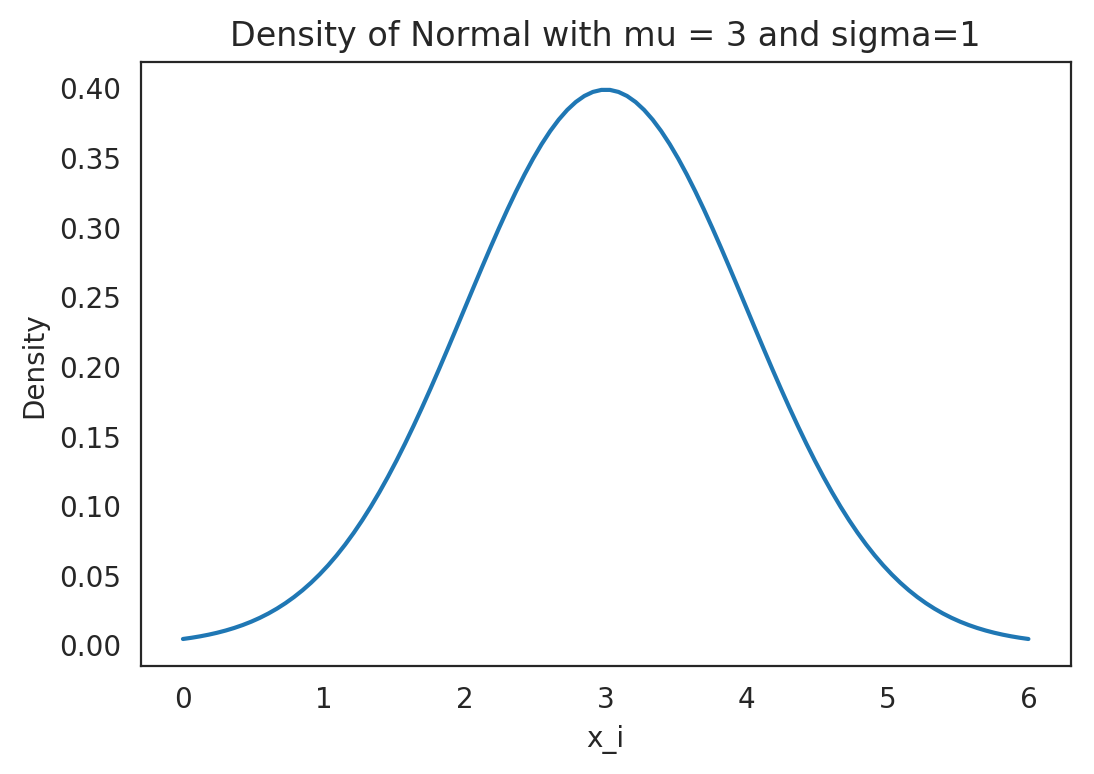
\includegraphics[width=\textwidth]{figures/normal_density.png}
    \end{figure}
\end{frame}


\begin{frame}[c]\frametitle{Basic Idea of Maximum Likelihood}
    \begin{equation}
        f(y_i) = \frac{1}{\sqrt{2\pi\sigma^2}} e^{\left(-\frac{1}{2 \sigma^2}(y_i - \mu)^2\right)} = \phi(y_i, \mu, \sigma) = l_i(\mu, sigma)
    \end{equation}
    \begin{itemize}
        \item $l$ is the likelihood contribution of individual $i$
        \item Interpretation: $y_i$ is fixed, $\mu$ and $\sigma$ vary
        \item Likelihood of whole sample is just product of individual likelihoods
        \item Use the parameters that maximize the likelihood of the sample as estimates
    \end{itemize}
\end{frame}


% \defverbatim[colored]\exampleCode{
% \begin{pythoncode}
%
%     import numpy as np
%     import pylab as pl
%
% \end{pythoncode}
% }
%
%
% \begin{frame}[c]\frametitle{title}
%     \exampleCode
% \end{frame}


\defverbatim[colored]\exampleCode{
\begin{pythoncode}

    import numpy as np
    import scipy

    def likelihood(mu, sigma, sample):
        likelihoods = scipy.stats.norm.pdf(sample, loc=mu, scale=sigma)
        return np.prod(likelihoods)

\end{pythoncode}
}

\begin{frame}[c]\frametitle{Python Implementation}
    \exampleCode
\end{frame}

\begin{frame}[c]\frametitle{Notebook}
    Look at likelihood\_example\_1.ipynb
\end{frame}


\begin{frame}[c]\frametitle{Some Insights from the Example}
    \begin{itemize}

        \item Use log-likelihood to avoid numerical problems
        \item Likelihood estimates can be counter-intuitive
        \item Larger sample -> more curved likelihood -> more precision
        \begin{itemize}
            \item Standard errors will depend on curvature of likelihood
        \end{itemize}
        \item Mean is estimated quite precisely, even in small samples
    \end{itemize}
\end{frame}


\begin{frame}[c]\frametitle{A Note on Terminology}
    \begin{itemize}
        \item Parameters are constants, not random variables
        \item Maximum likelihood estimates are not ``the most likely parameters''
        \item They a the parameter values that make the observed sample most likely!
    \end{itemize}
\end{frame}




\subsection{Method of Simulated Moments}


\begin{frame}[c]\frametitle{Basic Idea}
        \begin{itemize}
            \item Remember: If we have a fully parametric model and a parameter vector, we can simulate a dataset generated by the model with that parameter vector
            \item For the true parameter vector, simulated and observed sample should be similar
            \item MSM: Take the parameter vector that produces the dataset which is most similar to the empirical data as estimate
        \end{itemize}
\end{frame}


\begin{frame}[c]\frametitle{What Does Similar Mean?}
    \begin{itemize}
        \item Depends on the model
        \item Typically: Key moments are similar
        % \item Indirect Inference: moments are replaced by parameters of auxiliary model
        \item Selection of key moments depends on model
        \item Requires weighting matrix
    \end{itemize}
\end{frame}



\begin{frame}[c]\frametitle{Example 1: Which moments}
    \begin{itemize}
        \item Key moments: unconditional mean and variance
        \item Looks like chicken-or-egg problem
        \item Only an artifact of very simple example
    \end{itemize}
\end{frame}


\begin{frame}[c]\frametitle{Example 1: Objective function}
    \begin{itemize}
         \item empirical sample: $Y = y_1, y_2, \ldots, y_n$
         \item parameter vector: $\theta = (\mu, \sigma)^T$
         \item simulated sample, given $\theta$: $\hat{Y}^{\theta} = \hat{y}_1^{\theta}, \hat{y}_2^{\theta}, \ldots, \hat{y}_n^{\theta}$
         \item empirical moments: $m^{emp} = (mean(Y), var(Y))^T$
         \item simulated moments:  $m(\theta) = (mean(\hat{Y}^{\theta}), var(\hat{Y}^{\theta}))^T$
         \item Objective: $C(\theta) = (m(\theta) - m^{emp})^T W (m(\theta) - m^{emp})$
         \item $\theta^{MSM}$ minimizes this function
     \end{itemize}
\end{frame}



\defverbatim[colored]\exampleCode{
\begin{pythoncode}

    import numpy as np
    import scipy

    def msm_criterion(mu, sigma, sample):
        simulated_sample = np.random.normal(loc=mu, scale=sigma, size=len(sample))
        m_emp = np.array([[sample.mean()], [sample.std()]])
        m_sim = np.array([[simulated_sample.mean()], [simulated_sample.std()]])
        diff = m_emp - m_sim
        w = np.eye(2)
        return diff.T.dot(w).dot(diff)[0][0]

\end{pythoncode}
}

\begin{frame}[c]\frametitle{Python Implementation}
    \exampleCode
\end{frame}



\begin{frame}[c]\frametitle{Notebook}
    Look at msm\_example\_1.ipynb
\end{frame}





\begin{frame}[c]\frametitle{Some Insights from the Example}
    \begin{itemize}
        \item Precision is now limited by two factors:
        \begin{itemize}
            \item Sample variation
            \item Simulation noise
        \end{itemize}
        \item Likelihood needs the same assumption and will always be more efficient!
    \end{itemize}
\end{frame}


\begin{frame}[c]\frametitle{Why Would We Ever Use MSM?}
\begin{itemize}
    \item Likelihood often involves high dimensional integrals
    \item Likelihood is harder to derive
    \item Some say, MSM is more transparent
    \item Data might be on a slow server
    \item Different datasets
\end{itemize}
\end{frame}



\section{Numerical Optimization}


\begin{frame}[c]\frametitle{Why Numerical Optimization}
    \begin{itemize}
        \item Typically optimum cannot be calculated in closed form
        \begin{itemize}
            \item Derivatives are too complicated to evaluate
            \item Non differentiable functions
            \item First order conditions are too complicated
        \end{itemize}
        \item Numerical optimization works in these cases but:
        \begin{itemize}
            \item Typically no guarantee of global optimum
            \item Can be slow
            \item Less precise than closed form
        \end{itemize}
        \item WLOG, from now on only talk about minimization
    \end{itemize}
\end{frame}



\begin{frame}[c]\frametitle{We Already did it}
    \begin{itemize}
        \item For surface plots, we evaluated objective over whole reasonable parameter space
        \item Know coordinates of optimum
        \item This methods is called grid search or brute force
        \item Infeasible for high dimensional parameter vectors:
        \begin{itemize}
            \item Grid with 100 points in each dimension
            \item 50 parameters
            \item[$\rightarrow$] Criterion has to be evaluated at $10^{100}$ gridpoints
        \end{itemize}
        \item Need smarter algorithms to save evaluations!
    \end{itemize}
\end{frame}



\begin{frame}[c]\frametitle{Gradient Based vs. Gradient Free}
    \begin{itemize}
        \item Gradient based algorithms
        \begin{itemize}
            \item Require differentiable objective functions
            \item Use first derivative to determine direction of step
            \item Use second derivative to determine length of step
            \item Need much fewer function evaluations
        \end{itemize}
        \item Gradient free algorithms
        \begin{itemize}
            \item Work with non-smooth functions
            \item Basically a trial-and-error approach
        \end{itemize}
    \end{itemize}
\end{frame}



\begin{frame}[c]\frametitle{Termination Criteria}
    \begin{itemize}
        \item
    \end{itemize}
\end{frame}


\begin{frame}[c]\frametitle{Local vs. Global Optimizers}
    \begin{itemize}
        \item Local Optimizers:
        \begin{itemize}
            \item Start from start parameters and go down-hill
            \item Stop in first local minimum
        \end{itemize}
        \item Genetic Algorithms (typically global):
        \begin{itemize}
            \item Need bounds on parameter space
            \item Sample uniformly from parameters space to get start population
            \item Evolve to next generation by:
            \begin{itemize}
                 \item Killing worst parameters
                 \item Produce offspring of good parameters
            \end{itemize}
        \end{itemize}
        \item Pseudo global optimizers:
        \begin{itemize}
            \item Do local optimization from random start values
        \end{itemize}
    \end{itemize}
\end{frame}



\begin{frame}[c]\frametitle{Notebook}
    look at 1d\_minimization.ipynb
\end{frame}


\begin{frame}[c]\frametitle{Insights from the Example}

    \begin{itemize}
        \item Sampling scheme can be very important
        \item Robust optimizers can solve some problems, but maybe you don't need them!
        \item Always understand the problem you want to solve!
    \end{itemize}

\end{frame}



\defverbatim[colored]\exampleCode{
\begin{pythoncode}

    import numpy as np
    import scipy

    def smooth_msm_criterion(mu, sigma, sample):
        np.random.seed(5471)
        simulated_sample = np.random.normal(size=len(sample)) * sigma + mu
        m_emp = np.array([[sample.mean()], [sample.std()]])
        m_sim = np.array([[simulated_sample.mean()], [simulated_sample.std()]])
        diff = m_emp - m_sim
        w = np.eye(2)
        return diff.T.dot(w).dot(diff)[0][0]

\end{pythoncode}
}

\begin{frame}[c]\frametitle{Smooth Python Implementation}
    \exampleCode
\end{frame}


\section{Monte Carlo Results}


\begin{frame}[c]\frametitle{Notebook}

look at monte\_carlo.ipynb

\end{frame}


\section{Some Theory}


\begin{frame}[c]\frametitle{Closed Form Solution for Likelihood Function in Example 1}
    \begin{align*}
        L(\mu, \sigma) &= \prod_{i = 1}^n \frac{1}{\sqrt{2 \pi \sigma}} e^{\left(-\frac{1}{2 \sigma^2}(y_i - \mu)^2\right)} & \quad \text{Likelihood}\\
        \ell (\mu, \sigma) &= \sum_{i = 1}^n - \frac{1}{2}ln(2\pi\sigma) - \frac{1}{2 \sigma^2}(y_i - \mu)^2 & \quad \text{Log-Likelihood} \\
        \frac{\partial \ell}{\partial \mu} &= \frac{1}{\sigma^2} \sum_{i = 1}^n (y_i - \mu) \stackrel{!}{=} 0 & \quad \text{FOC} \\
        \mu^{*} &= \frac{1}{n} \sum_{i = 1}^n y_i
    \end{align*}
\end{frame}


\begin{frame}[c]\frametitle{Example 2: Linear Model}
    \begin{itemize}
        \item Dataset: iid sample of variables $y_i$, $x_i$
        \item Model: $y_i = x_i'\beta + u_i$, $u_i \sim \mathcal{N}(0, \sigma^2)$
        \item Parameters to estimate: $\beta, \sigma$
        \pause
        \item You might be tempted to call this an OLS model
        \item Later you'll see why this is not a good idea
    \end{itemize}
\end{frame}


\begin{frame}[c]\frametitle{Likelihood Function of Linear Model}
    \begin{align*}
        f(y_i \mid \beta, \sigma, x_i) &= \frac{1}{\sqrt{2\pi\sigma^2}} e^{\left(-\frac{1}{2 \sigma^2}(y_i - x_i' \beta)^2\right)} \\
        L(\beta, \sigma) &= \prod_{i = 1}^n f(y_i \mid \beta, \sigma, x_i)
    \end{align*}

    \vspace{1cm}
    \begin{itemize}
        \item Take logs
        \item Set FOCs to zero
        \item If you make no mistake, you will see that $\beta^{*}$ equals the OLS estimator
    \end{itemize}
\end{frame}


\begin{frame}[c]\frametitle{The Deep Reason (simplified!)}
\begin{itemize}
    \item It can be shown that:
    \begin{itemize}
        \item Maximum Likelihood is asymptotically efficient
        \item No unbiased estimator has smaller variance than maximum likelihood (Cramér-Rao Bound)
    \end{itemize}
    \item From Gauss Markov Theorem we know:
    \begin{itemize}
        \item OLS estimator is Best Linear Unbiased Estimator
        \item Remember: sample mean = OLS on constant
    \end{itemize}
    \item Since OLS and Maximum Likelihood estimators are both optimal, they have to coincide
\end{itemize}
\end{frame}


\begin{frame}[c]\frametitle{MSM of Linear Model}
    \begin{itemize}
        \item Identifying assumption: $u_i$ is uncorrelated with $x_i$
        \item $E(x_i u_i) = E(x_i (y_i - x_i' \beta)) = 0$
        \item Gives us $k$ moment conditions for $k$ parameters
        \item Those are the moments used when Linear model is estimated with GMM
        \item Could use the simulated version of those moments to estimate Linear model with MSM
        \item Reminder: This is just to explain the method
    \end{itemize}
\end{frame}
% standard errors
% equality of OLS and ML for normal linear model
% equality of OLS, sample mean and ML for normal mean model
% weighting matrices






\section{Estimagic}



\begin{frame}[c]\frametitle{Estimagic}
    \begin{itemize}
        \item Wrap local, global and pseudo global optimizers from Pygmo, Scipy and TAO
        \item Standard errors for likelihood and MSM models
        \item Elegant interface for typical constraints
        \begin{itemize}
            \item e.g. estimate covariance matrices, probabilities, \ldots
        \end{itemize}
        \item Interactive dashboard with live convergence plots
    \end{itemize}
\end{frame}



\begin{frame}[c]% \frametitle{title}
    \begin{figure}
        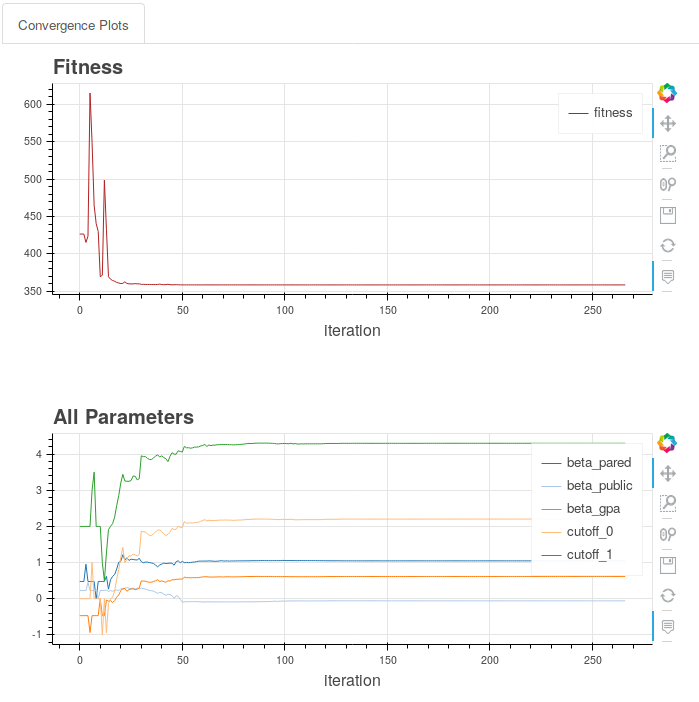
\includegraphics[height=\textheight]{figures/convergence_plot.png}
    \end{figure}
\end{frame}


\begin{frame}[c]\frametitle{Some Tipps}
    \begin{itemize}
        \item Start by implementing toy examples
        \item When you hit problem, reproduce and solve them in minimal examples
        \item Use as much existing code as possible
        \item If you think you need a fancy optimizer, you probably don't
        \item If you ever do structural econometrics: use estimagic!
        \item But maybe wait a few months \ldots
    \end{itemize}
\end{frame}



% \appendix
% \begin{frame}[allowframebreaks]
%     \frametitle{References}
%     \renewcommand{\bibfont}{\normalfont\footnotesize}
%     \printbibliography
% \end{frame}

\end{document}


